\documentclass{article}

\usepackage[ngerman]{babel}
\usepackage[utf8]{inputenc}
\usepackage[T1]{fontenc}
\usepackage{hyperref}
\usepackage{csquotes}
\usepackage{graphicx}
\usepackage{float}
\usepackage{caption}

\usepackage[
    backend=biber,
    style=apa,
    sortlocale=de_DE,
    natbib=true,
    url=false,
    doi=false,
    sortcites=true,
    sorting=nyt,
    isbn=false,
    hyperref=true,
    backref=false,
    giveninits=false,
    eprint=false]{biblatex}
\addbibresource{../references/bibliography.bib}

\title{Notizen zu KI in der Medizin}
\author{Käthe Linke Aguirre}
\date{\today}

\begin{document}
\maketitle

\abstract{
    Dieses Dokument ist eine Sammlung von Notizen zu dem Projekt. Die Struktur innerhalb des
    Projektes ist gleich ausgelegt wie in der Hauptarbeit, somit kann hier einfach geschrieben
    werden, und die Teile die man verwenden möchte, kann man direkt in die Hauptdatei ziehen.}

    \tableofcontents

\newpage

\section{Die Künstliche Intelligenz}


\subsection{Definition von KI}
  
Künstliche Intelligenz (KI) ist die Fähigkeit einer Maschine, menschliche Fähigkeiten
wie logisches Denken, Lernen, Planen und Kreativität zu imitieren. KI ist einer der 
großen technologischen Fortschritte unserer Zeit. Ihre Entwicklung schreitet 
rasant voran und die Einsatzmöglichkeiten nehmen zu. KI ist ein wichtiger Bestandteil nicht nur in der Informatik,
sondern auch vieler anderer Bereiche unseres Lebens. 
\newline
KI wird zum Beispiel,... 
\begin{enumerate}
    \item in der Bildung verwendet. Adaptive Lernplatformen wie Knewton, Quizlet und Duolingo bildet bieten Nutzer individuelle Lernsysteme. Sie können mit automatisierte Tutoren, die Schülern bei ihren Aufgaben helfen.
    \item in der Architektur verwendet. Sie kann zum Beispiel Gebäudeentwürfe generieren.
    \item in der Kunst verwendet. KI kann mithilfe von generative Modelle, Kunstwerke erstellen oder auch mit KI-Programme, Musik komponieren.
\end{enumerate}

Auch in der Medizin spielt KI eine bedeutende Rolle. In meinem Dokument werde ich mich
mit dem Einsatz von Künstlicher Intelligenz beschäftigen und ob dieser Einsatz
ethisch vertretbar ist oder nicht. 

\subsection {Wie wird KI trainiert?}

KI-Modelle werden in der Regel durch einen Prozess des maschinellen Lernens trainiert, der in drei Hauptschritte unterteilt werden kann.  Der Trainingprozess beginnt mit der Datensammung, bei der ein Computeralgorithmus mit einer grossen Menge an Daten gefüttert wird , die für die Erstellung von Vorhersagen und deren Genauigkeit notwendig sind. Diese Daten können strukturiert (z.B. Tabellen) oder unstrukturiert (z.B. Texte) sein.Während des Trainings wird das Modell beigebracht, verschiedene Merkmale in den Daten zu erkennen, indem es seine internen Parameter anpasst, um Fehler bei der Vorhersage zu minimieren. Im zweiten Schritt findet ein Validierungsprozess statt, bei dem bewertet wird, wie gut das trainierte Modell zuvor ungesehene Daten abschneidet. Schliesslich wird das Modell mit neuen, bisher ungesehenen Daten getestet, um zu überprüfen, ob es genaue Vorhersahen treffen kann oder nicht. 
\citep{clickworker}
\newline
Jedoch ist zu beachten, dass bei der Datensammlung und Datenverwendeung, Datenschutzrichtlinien und -gesetze eingehalten werden, um zu sicherzustellen, dass die Privatsphäre und die Rechte von Personen respektiert werden. Ein anderer wichtiger Aspekt, dass beachtet werden sollte, ist das die Funktionsweise und die Entscheidungen, die das System trifft, verständlich und nachvollziehbar ist. Ist das nicht der Fall, dann können Probleme wie Skepsis und Ablehnung auftreten. 


\section{KI in der Medizin}


\subsection{Wie wird KI in der Medizin verwendet?}

Künstliche Intelligenz (KI) wird im Gesundheitsbereich in verschiedenen Bereichen 
eingesetzt. Es gibt welche die Nicht-Medizinprodukte und Medizinprodukte sind. 



Sie wird verwendet um Krankheiten zu diagnostizieren, potenziell bösartige Läsionen oder 
gefährliche Herzmuster zu markieren und Ärzte bei der Interpretation dieser Signale zu unterstützen. 
Außerdem kann KI genutzt werden, um relevante Muster in digitalisierten medizinischen 
Daten zu finden und präzise Entscheidungen zu treffen. 

\begin{figure}[H]
    \centering
    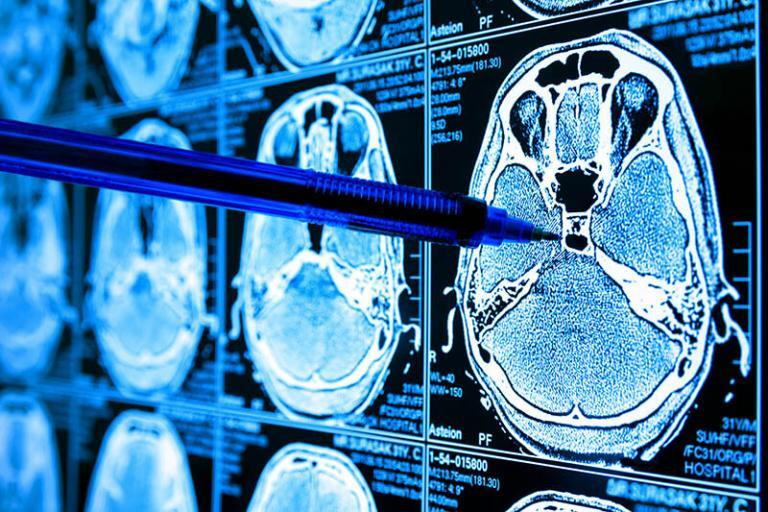
\includegraphics[width=0.5\textwidth]{kimedizin.jpg}
    \caption{Random}
    \label{fig:kimedizin}
\end{figure}



\subsection {Welche Probleme können vortreten? Ist es ethisch vertretbar?}


\subsection{Kann die KI Ärzte ersetzten?}

\section {Zitat}






\input{section_ai.tex}

\printbibliography

\end{document}
